% -------------------------------------------------------------------
\documentclass[usepdftitle=false,handout,10pt]{beamer}

%encodings
\usepackage[utf8]{inputenc}
\usepackage[OT1]{fontenc}

%some useful packages
\usepackage[]{mathrsfs}
\usepackage[]{amssymb}
\usepackage[]{amsmath}
\usepackage[]{acronym}
\usepackage[]{listings}
\usepackage[]{xcolor}
\usepackage[]{graphicx}
\usepackage[]{textcomp} %for tilde


\renewcommand{\matrix}[1]{\boldsymbol{#1}}
\renewcommand{\vector}[1]{\boldsymbol{#1}}
\renewcommand{\d}{\mathrm{d}}
\newcommand{\domelem}[1]{\boldsymbol{\mathrm{#1}}}
\newcommand{\kB}{k_\mathrm{B}}
\newcommand{\VT}{V_\mathrm{T}}
\newcommand{\q}{\mathrm{q}}
\newcommand{\LandauO}{\mathcal{O}}


\graphicspath{{figures/}}           % in which folder all the figures are

% table of contents, depth
\setcounter{tocdepth}{2}

% modify at will
%\setbeamercovered{transparent}
\setbeamercovered{invisible}

%\usetheme[height=0.3cm,width=0.8cm,shadow=false]{iue}

\hypersetup{pdftitle   = {Semiconductor Device Simulation Approaches for Massively Parallel Computing Architectures},
            pdfsubject = {Computational and Numerical Methods in Electronics, SIAM CSE 2017},
            pdfauthor={Karl Rupp}}

\author[Karl Rupp]{\normalfont \underline{Karl Rupp}$^{1,2}$, Tibor Grasser$^{2}$, Ansgar J\"ungel$^{3}$}

\institute[TU Wien]
{ \footnotesize
  $^1$ Freelance Computational Scientist \\
  $^2$ Institute for Microelectronics \\
  $^3$ Institute for Analysis and Scientific Computing \\
  TU Wien, Austria  
}

\title[ViennaSHE]{Semiconductor Device Simulation Approaches\\ for Massively Parallel Computing Architectures}

\date[February 27th, 2017]{\footnotesize MS: Computational and Numerical Methods in Electronics \\ SIAM CSE, Atlanta, February 27th, 2017}

\setbeamertemplate{blocks}[default]
\setbeamercolor{block body}{bg=}

\begin{document}


\begin{frame}[plain]
 \frametitle{~}
 \titlepage
\end{frame}



\begin{frame} {Semiconductor Device Simulation} 
 \begin{block}{Selection of Semiclassical Models}
  \begin{itemize}
   \item Drift-diffusion model
   \item Hydrodynamic model
   \item Energy transport model
   \item ...
  \end{itemize}
 \end{block}

 \begin{center} 
  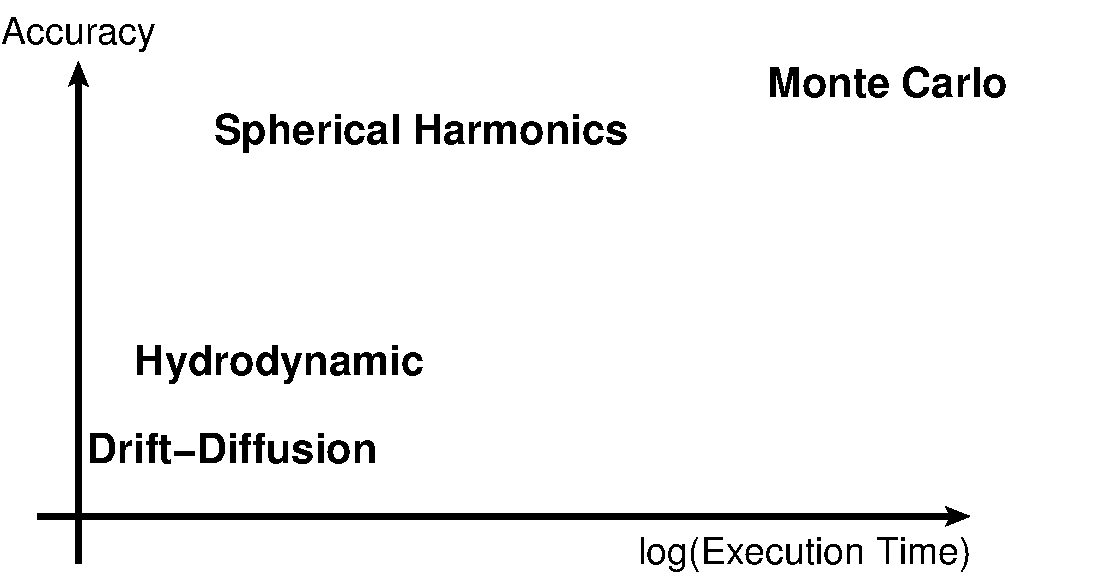
\includegraphics[width=0.6\textwidth]{simulation-comparison}
 \end{center}  
\end{frame} 


\begin{frame} {Scalability of Linear Solvers} 
 \begin{center} 
  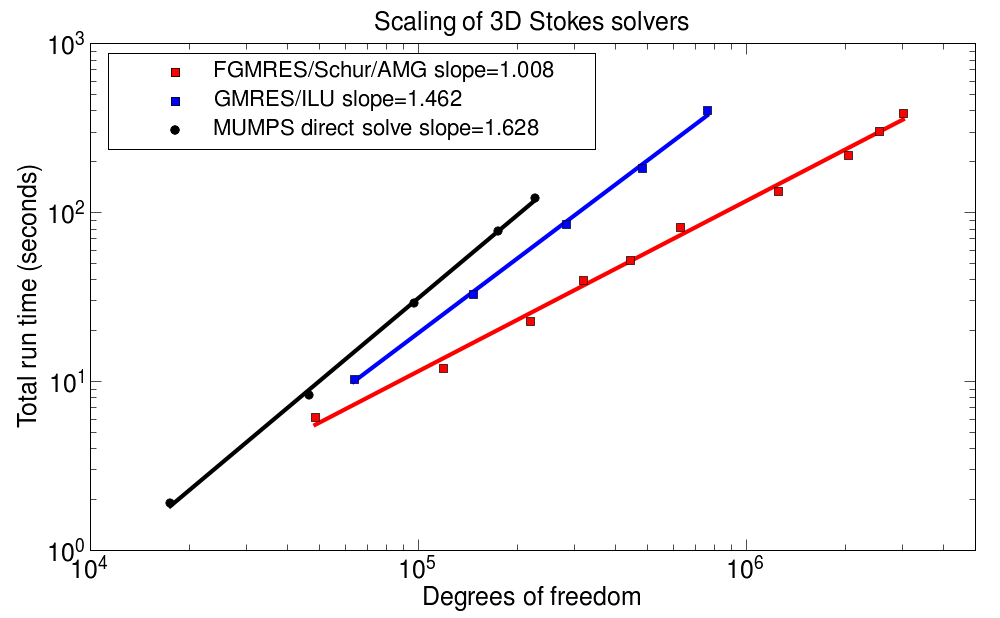
\includegraphics[width=0.96\textwidth]{StokesScalingDirectVsChebySchur} \\
  \footnotesize (courtesy of Jed Brown)
 \end{center}  
\end{frame} 


%\section*{Contents}

\begin{frame}{Contents}
  \begin{block}{The Spherical Harmonics Expansion Method}
   \begin{itemize}
    \item Comparison to Monte Carlo
    \item Shared-memory parallelization
    %\item Carrier-carrier scattering
   \end{itemize}
  \end{block}
  
  \begin{block}{Solution on Distributed Memory Machines}
   \begin{itemize}
    \item Preconditioner blueprints
    \item Node-level parallel ILU
   \end{itemize}
  \end{block}
  
\end{frame}


\begin{frame} {Semiconductor Devices in 3D: FinFET} 
  
 \begin{center} 
   {\footnotesize Intel Trigate transistors} \\
   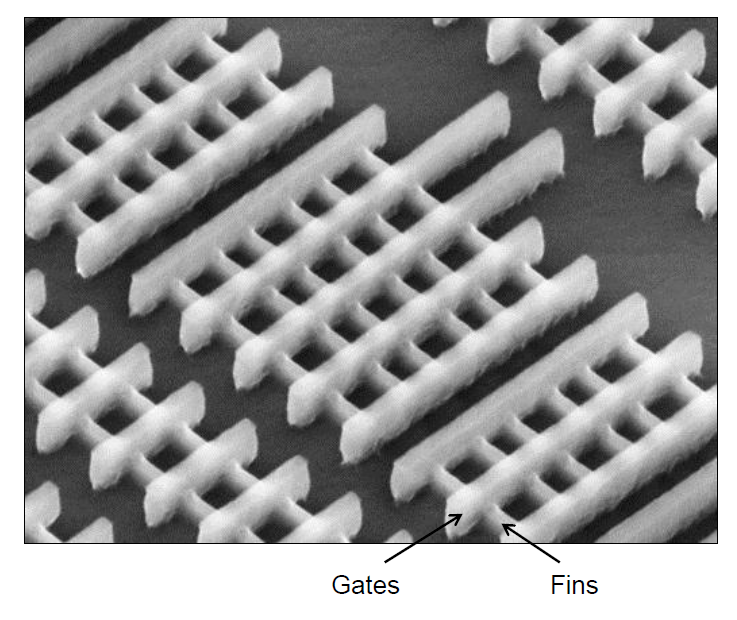
\includegraphics[width=0.7\textwidth]{intel-trigate}
 \end{center} 
 
\end{frame} 

% 
% \begin{frame} {Electron Density in a FinFET} 
%   
%  \begin{center} 
%   Density of electrons at each point $\vector x$ \\ 
%   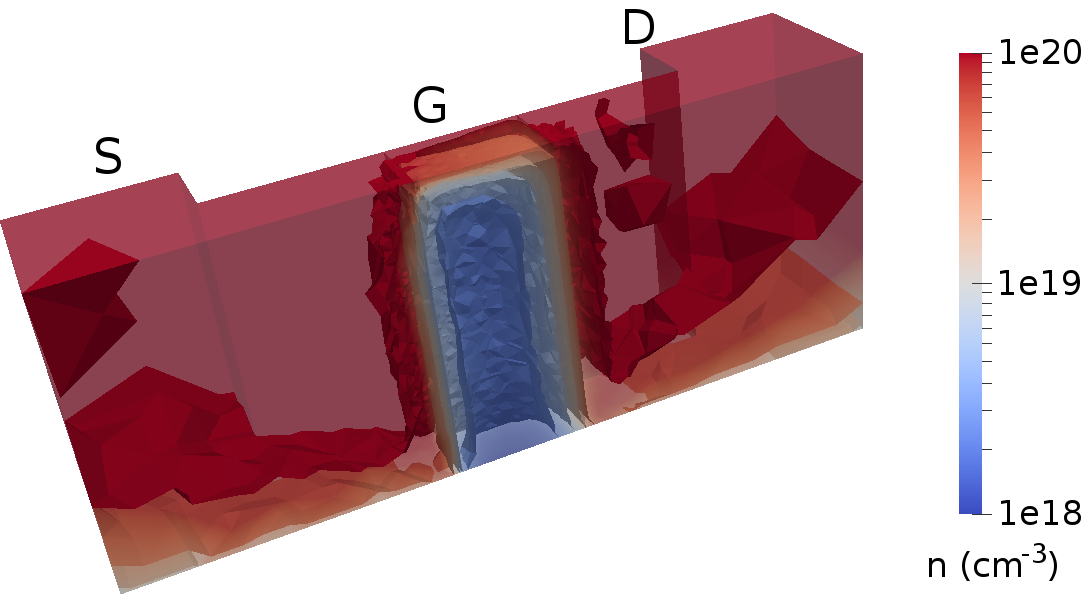
\includegraphics[width=0.632\textwidth]{trigate-electrons-mod}
%  \end{center} 
%   \vspace*{2.68cm}
%  
% \end{frame} 
%  
% 
% \begin{frame}{Electron Energy Distribution?} 
%  \begin{center} 
%   Distribution of electrons with respect to energy at $\vector x$? \\ 
%   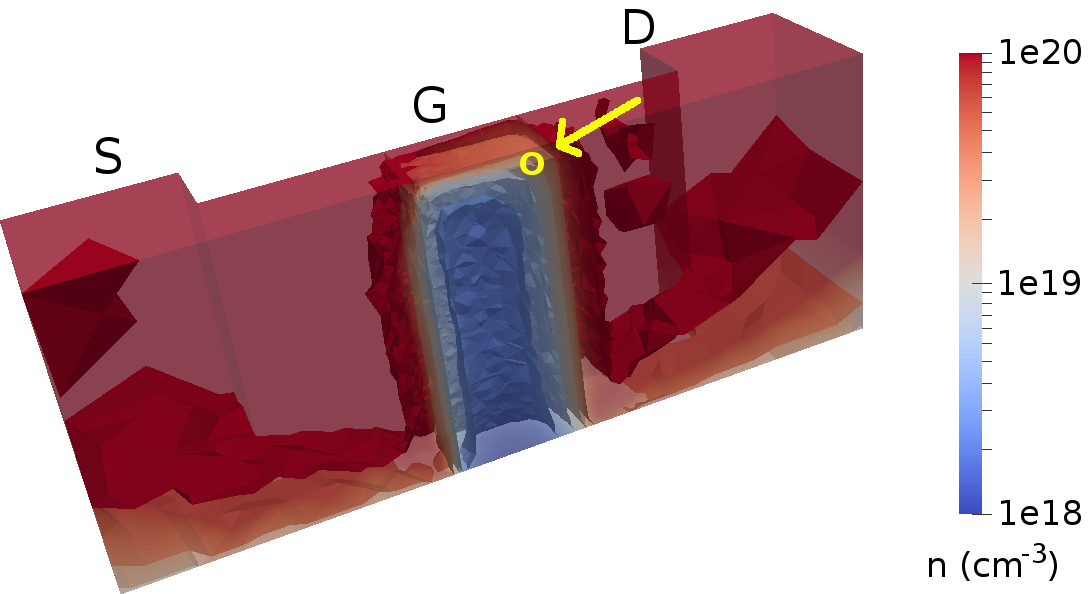
\includegraphics[width=0.632\textwidth]{trigate-electrons-mod2}
%  \end{center} 
%   \vspace*{2.68cm}
% \end{frame} 
%  
% \begin{frame} {Electron Energy Distribution?} 
%  \begin{center}Distribution of electrons with respect to energy at $\vector x$? \\ 
%   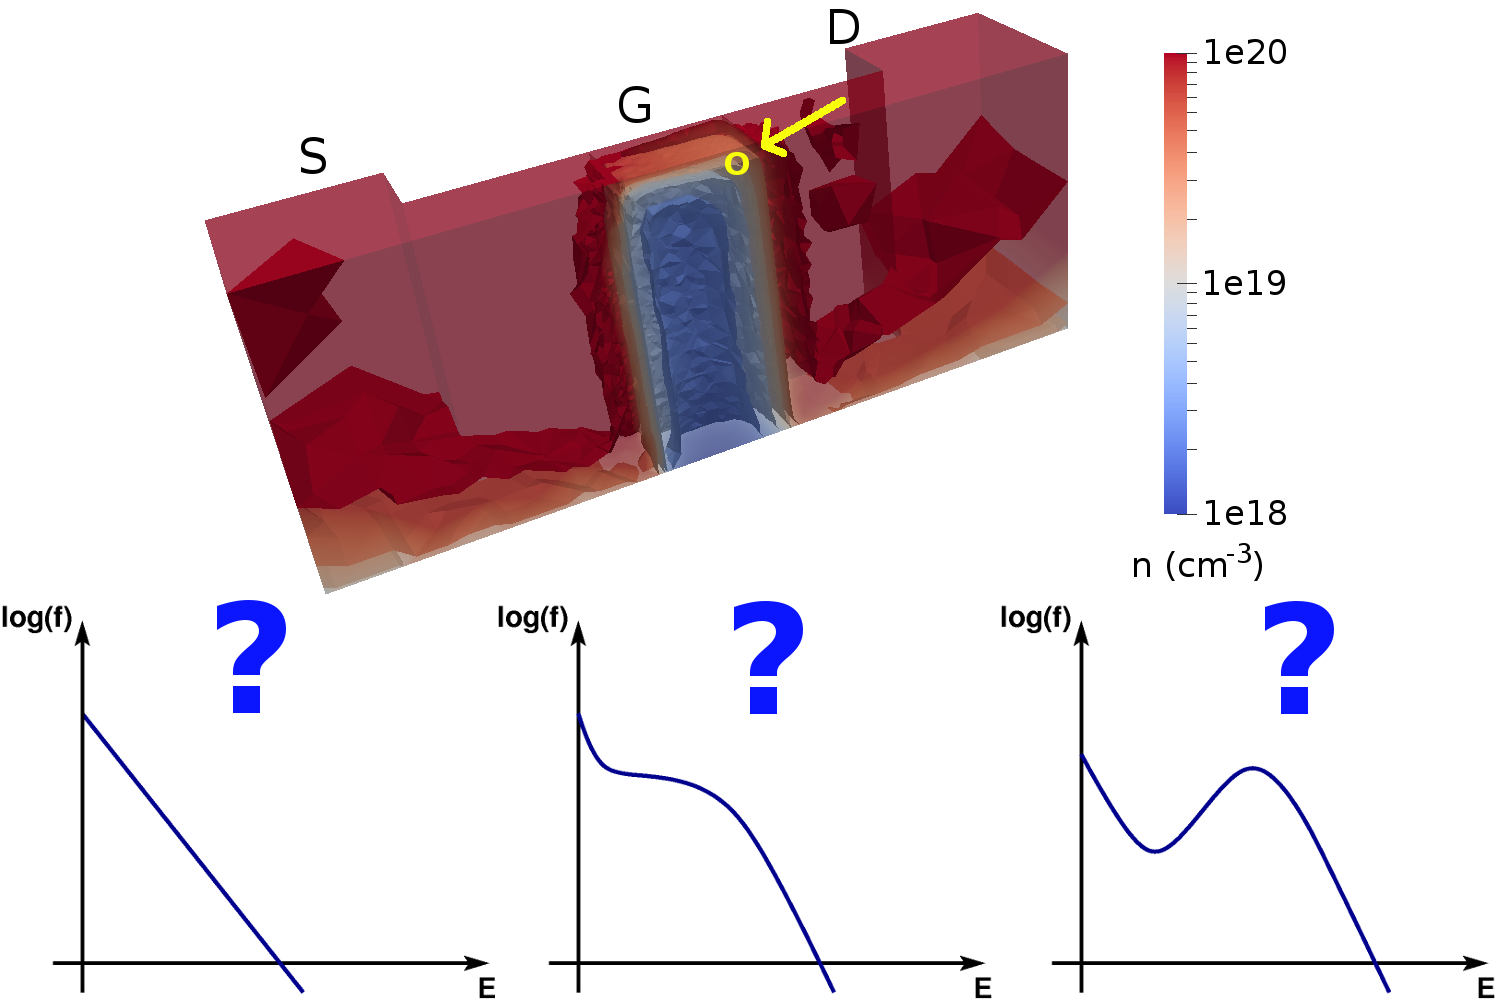
\includegraphics[width=0.87\textwidth]{trigate-electrons-edf-1}
%  \end{center} 
% \end{frame} 
%  
% \begin{frame} {Electron Energy Distribution?} 
%  \begin{center}Distribution of electrons with respect to energy at $\vector x$? \\ 
%   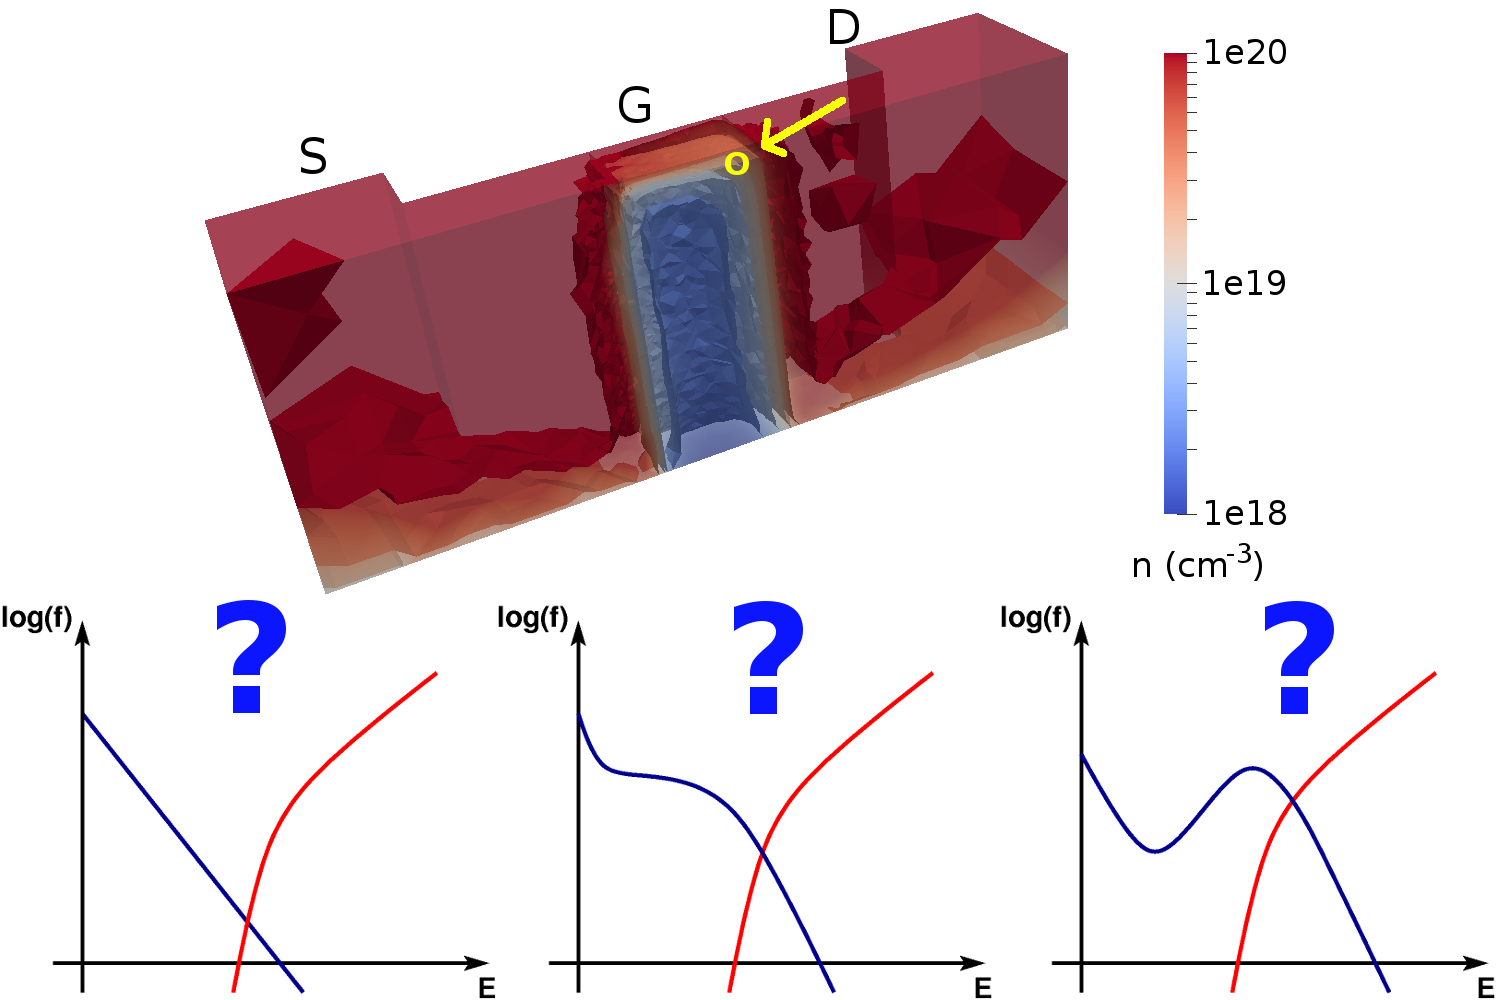
\includegraphics[width=0.87\textwidth]{trigate-electrons-edf-2}
%  \end{center} 
% \end{frame} 
%  
\begin{frame} {Electron Energy Distribution?} 
 \begin{center}Distribution of electrons with respect to energy at $\vector x$? \\ 
  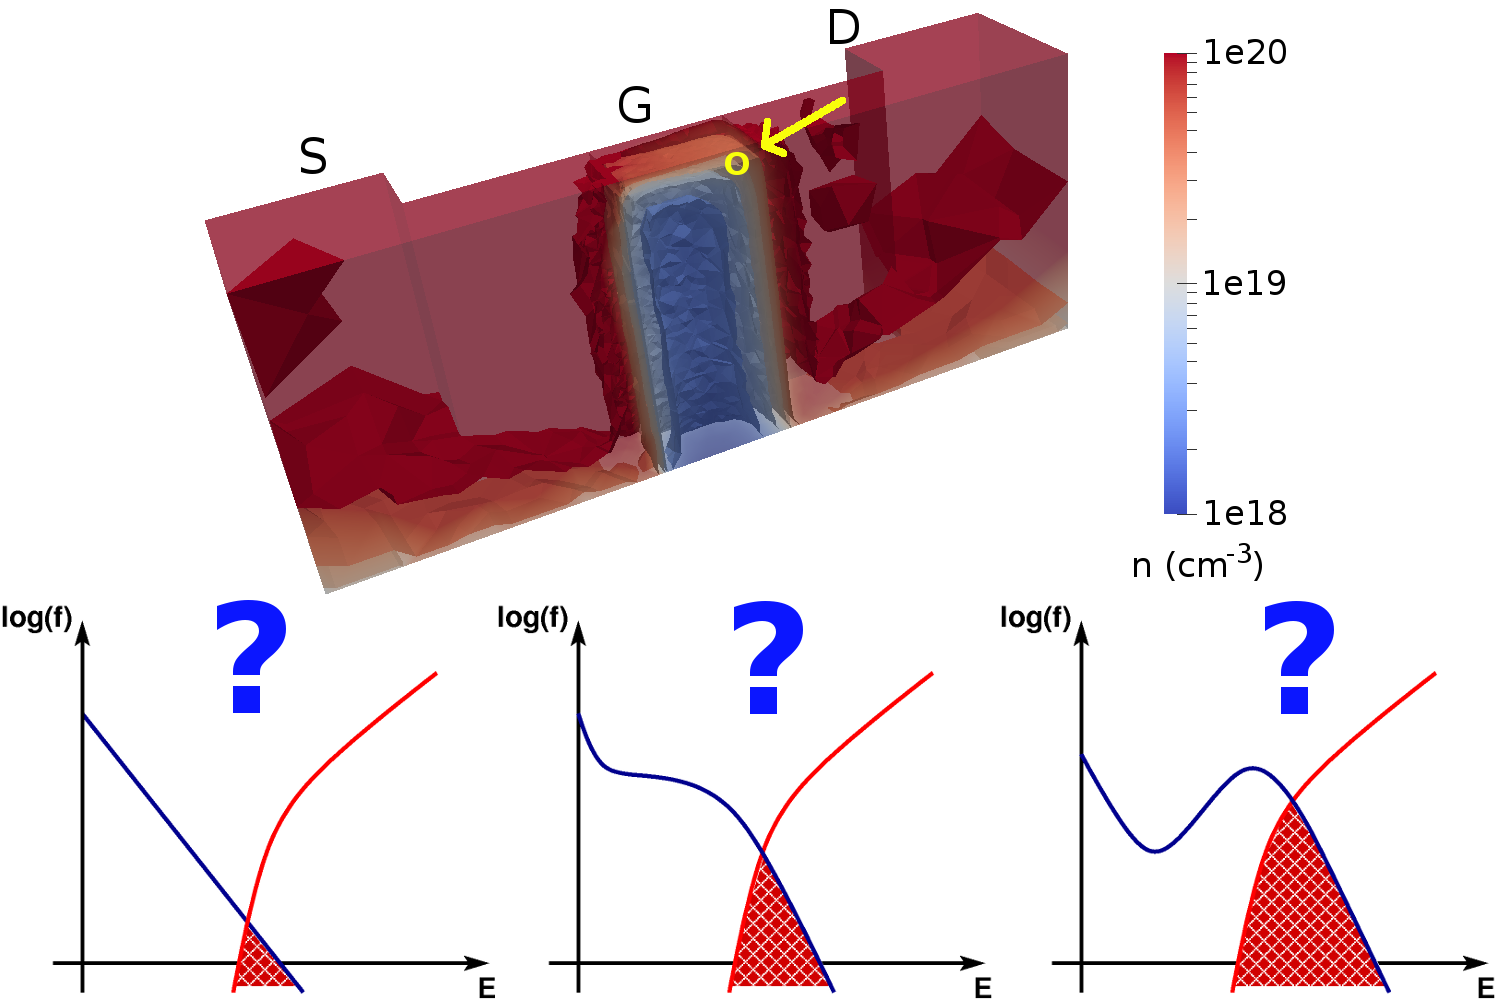
\includegraphics[width=0.87\textwidth]{trigate-electrons-edf-3}
 \end{center} 
\end{frame} 
 

 
% 
% \begin{frame} {Electron Energy Distribution?}
%  \begin{center}
%   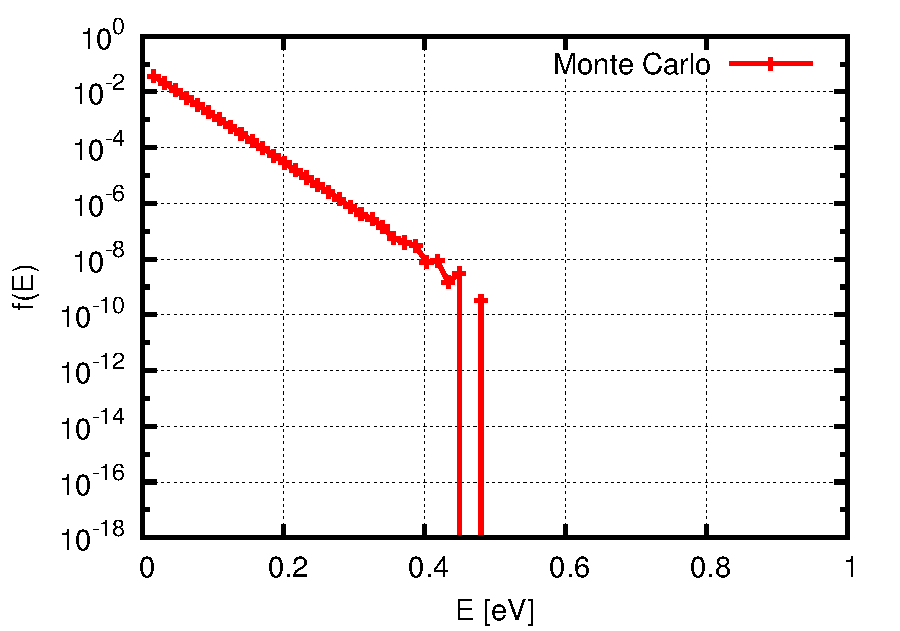
\includegraphics[width=0.95\textwidth]{she-monte-carlo-1}
%  \end{center}
% \end{frame}

\begin{frame} {Electron Energy Distribution?}
 \begin{center}
  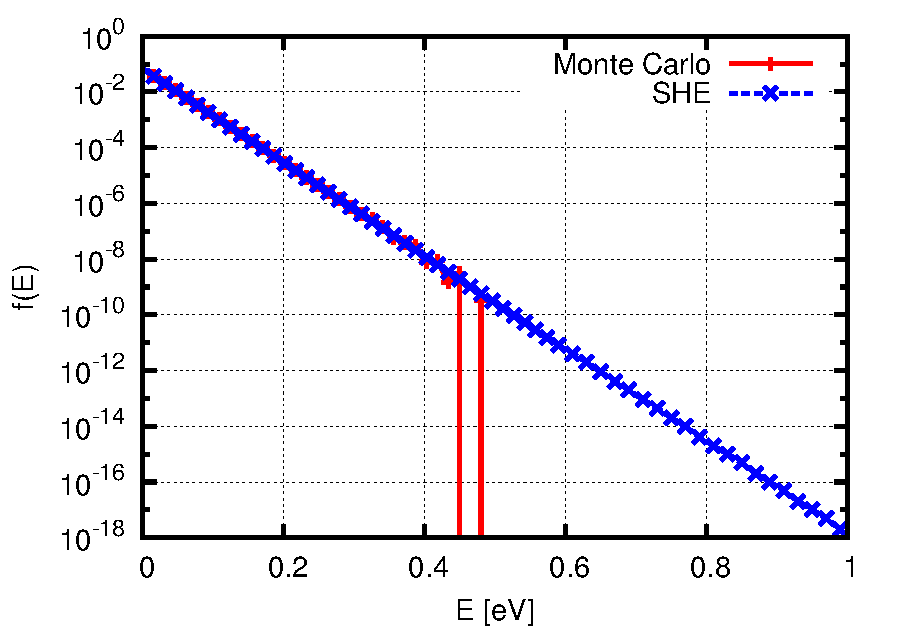
\includegraphics[width=0.95\textwidth]{she-monte-carlo-2}
 \end{center}
\end{frame}
 

\section{Spherical Harmonics Expansion Method}


\begin{frame}{Spherical Harmonics Expansion Method}

 \vspace*{-0.3cm}
  \begin{block}{Spherical Symmetries}
  \begin{itemize}
   \item Maxwell distribution of carriers at equilibrium
   \item Dispersion relation (Herring-Vogt transform, approx.)
  \end{itemize}
  \end{block}

  \vspace*{-0.5cm}
  \begin{block}{}
   \begin{itemize}
    \item 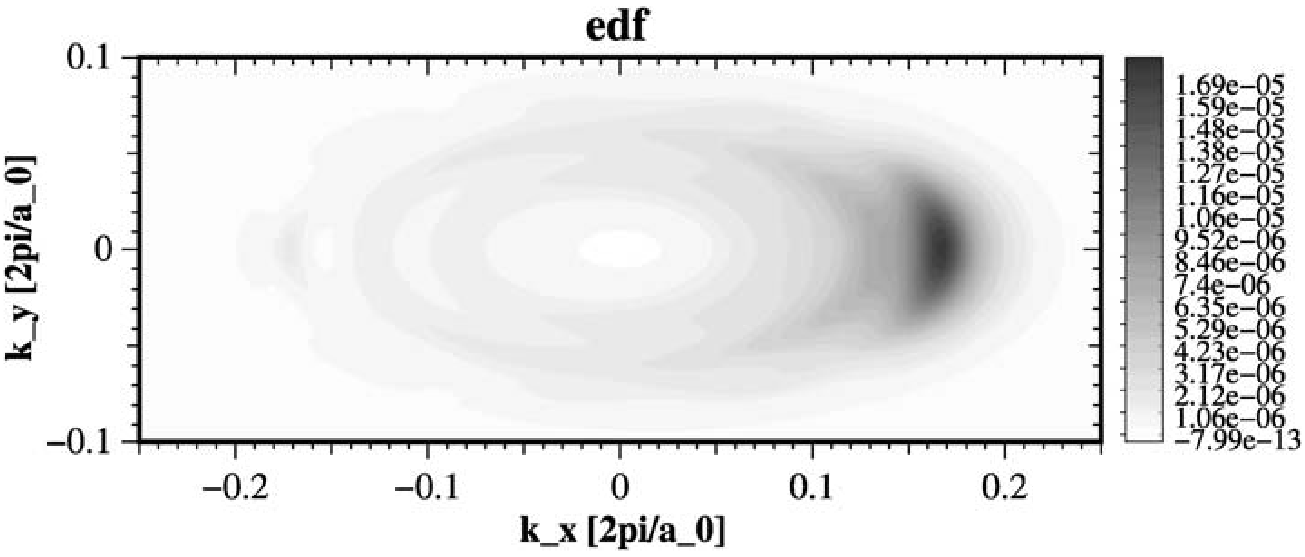
\includegraphics[width=0.78\textwidth]{edf}
    \item {\scriptsize \ S.-M.~Hong and C.~Jungemann (2009)}
   \end{itemize}
  \end{block}

\end{frame}


\begin{frame}{Spherical Harmonics Expansion Method}

 \vspace*{-0.3cm}
  \begin{block}{Spherical Symmetries}
  \begin{itemize}
   \item Maxwell distribution of carriers at equilibrium
   \item Dispersion relation (Herring-Vogt transform, approx.)
  \end{itemize}
  \end{block}

 
     \vspace*{0.62cm}
  \begin{block}{Spherical Harmonics Expansion (SHE)}
     \vspace*{-0.5cm}
      { %\Large
       \begin{align*}
	f(\vector x, \vector k, t) \simeq \sum_{l = 0}^L \sum_{m=-l}^l f_{l,m}(\vector x, E, t) Y_{l,m}(\theta, \varphi)
      \end{align*}}
     \vspace*{-0.5cm}
    \begin{itemize}
     \item New unknowns: $f_{l,m}(\vector x, E, t)$
     \item Solution in five-dimensional $(\vector x, E, t)$-space
     \item S.-M.~Hong and C.~Jungemann, \textit{J Comput Electron} (2009): \\
           Fifth-order, three-dim.~$(\vector x, E)$-space, 26 GB memory, 12 hours
    \end{itemize}
   \end{block}
%     \vspace*{-0.4cm}


\end{frame}




%
% Parallelization
%

\section{Parallelization}

\begin{frame}{Parallelization}
 \begin{block}{Preconditioner for Iterative Linear Solvers}
  \begin{itemize}
   \item No fast general-purpose parallel preconditioner available
   \item Physics-based parallel block preconditioner developed
  \end{itemize}
  \begin{center}
   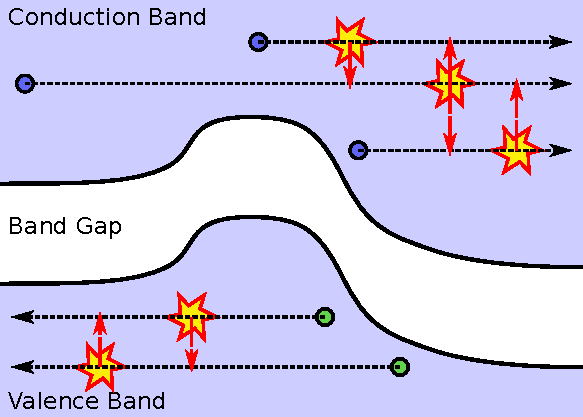
\includegraphics[width=0.7\textwidth]{htransformation}
  \end{center}
 \end{block}
%  \vspace*{-0.4cm}

\end{frame}


% 
% \begin{frame}{Parallelization}
%  \begin{block}{Scaling of Solution Variables}
%   \begin{itemize}
%    \item Exponential decay with energy: $f(E_i) \sim \exp(- \frac{E_i}{k_\mathrm{B} T})$
%    \item {\color{white} Rescale unknowns: $\tilde{f}(E_i) = \exp( \frac{E_i}{k_\mathrm{B} T}) f(E_i)$}
%    \item {\color{white} New system: $\tilde{\matrix A} \tilde{\vector x} = \matrix A \matrix D \matrix D^{-1} \vector x = \vector b$}
%    \item {\color{white} Row normalization: $\hat{\matrix A} \tilde{\vector x} = \matrix P \tilde{\matrix A} \tilde{\vector x} = \matrix P \vector b$}
%   \end{itemize}
%   \begin{center}
%    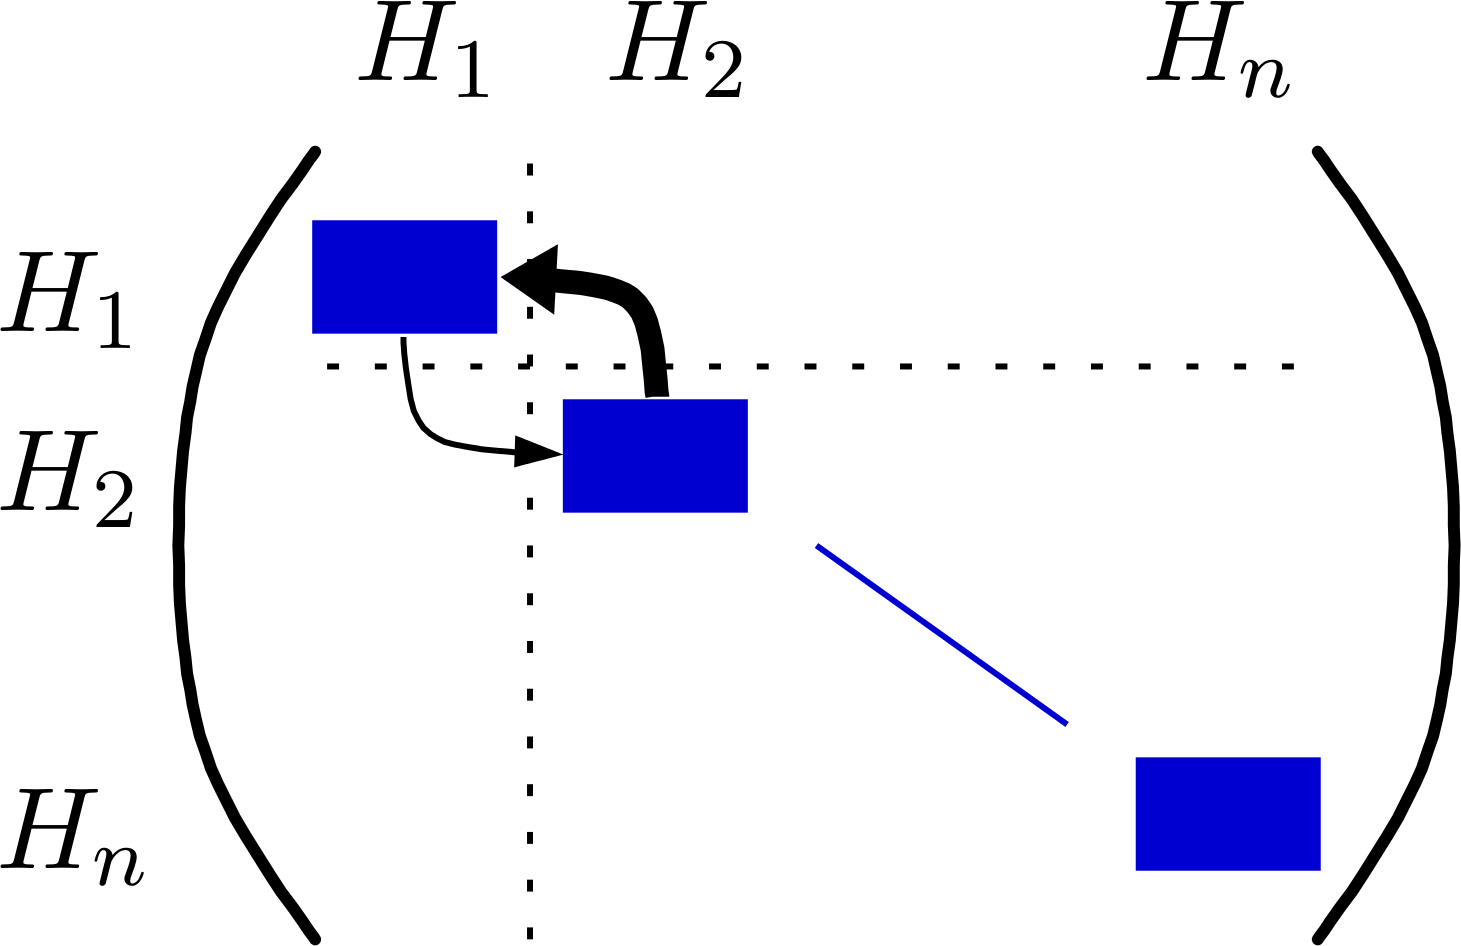
\includegraphics[width=0.45\textwidth]{matrix-structure-1} \hfill $\hphantom{1}$
%    %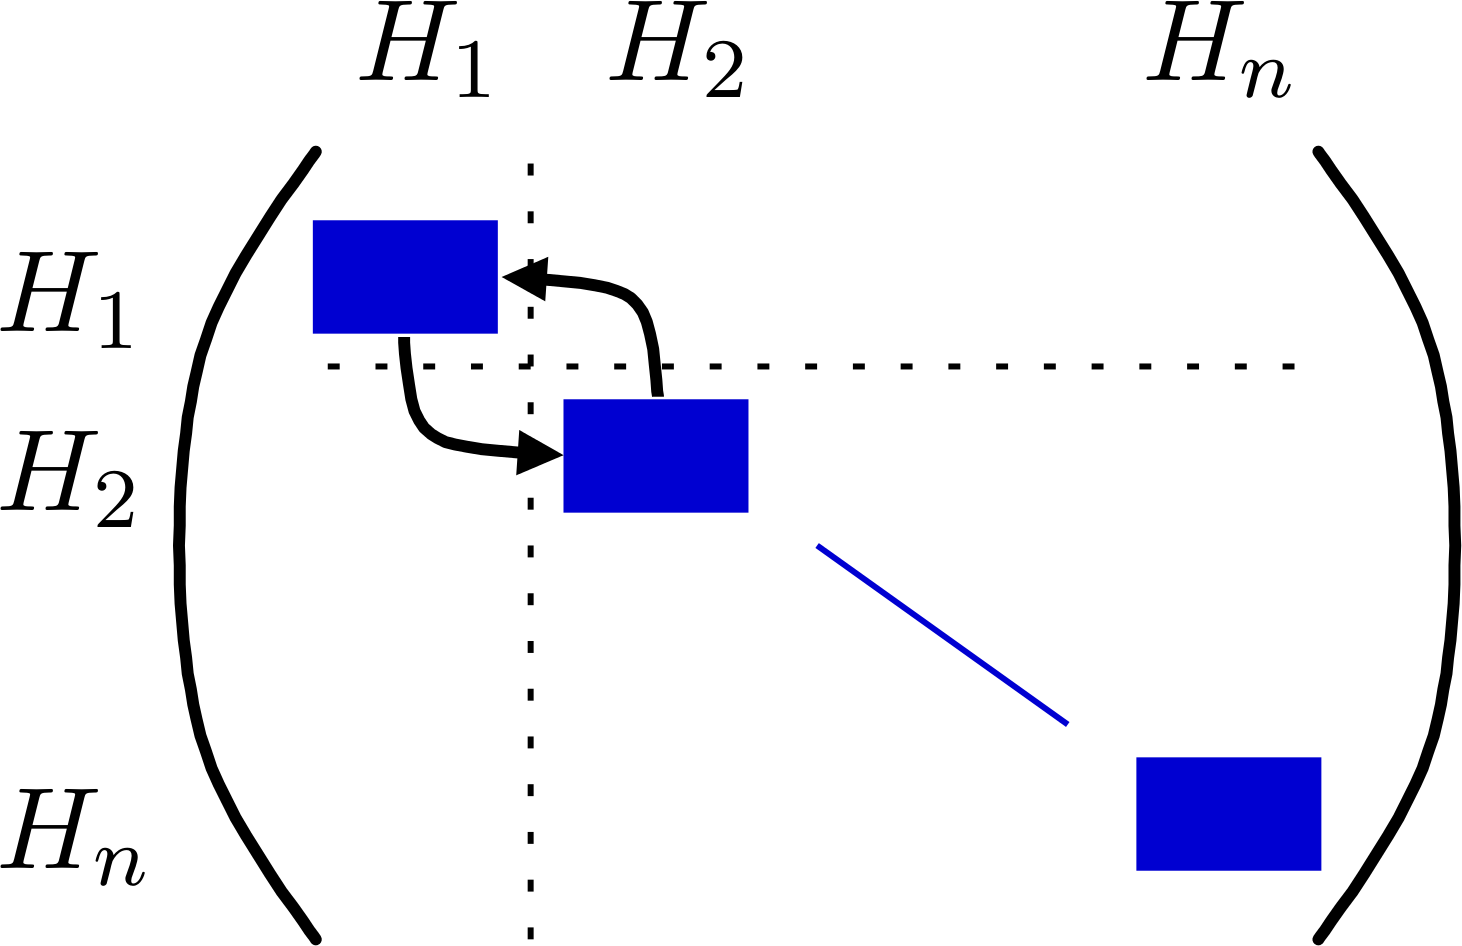
\includegraphics[width=0.45\textwidth]{matrix-structure-2}
%   \end{center}
%  \end{block}
% %  \vspace*{-0.4cm}
% 
% \end{frame}
% 
% 
% \begin{frame}{Parallelization}
%  \begin{block}{Scaling of Solution Variables}
%   \begin{itemize}
%    \item Exponential decay with energy: $f(E_i) \sim \exp(- \frac{E_i}{k_\mathrm{B} T})$
%    \item Rescale unknowns: $\tilde{f}(E_i) = \exp( \frac{E_i}{k_\mathrm{B} T}) f(E_i)$
%    \item {\color{white} New system: $\tilde{\matrix A} \tilde{\vector x} = \matrix A \matrix D \matrix D^{-1} \vector x = \vector b$}
%    \item {\color{white} Row normalization: $\hat{\matrix A} \tilde{\vector x} = \matrix P \tilde{\matrix A} \tilde{\vector x} = \matrix P \vector b$}
%   \end{itemize}
%   \begin{center}
%    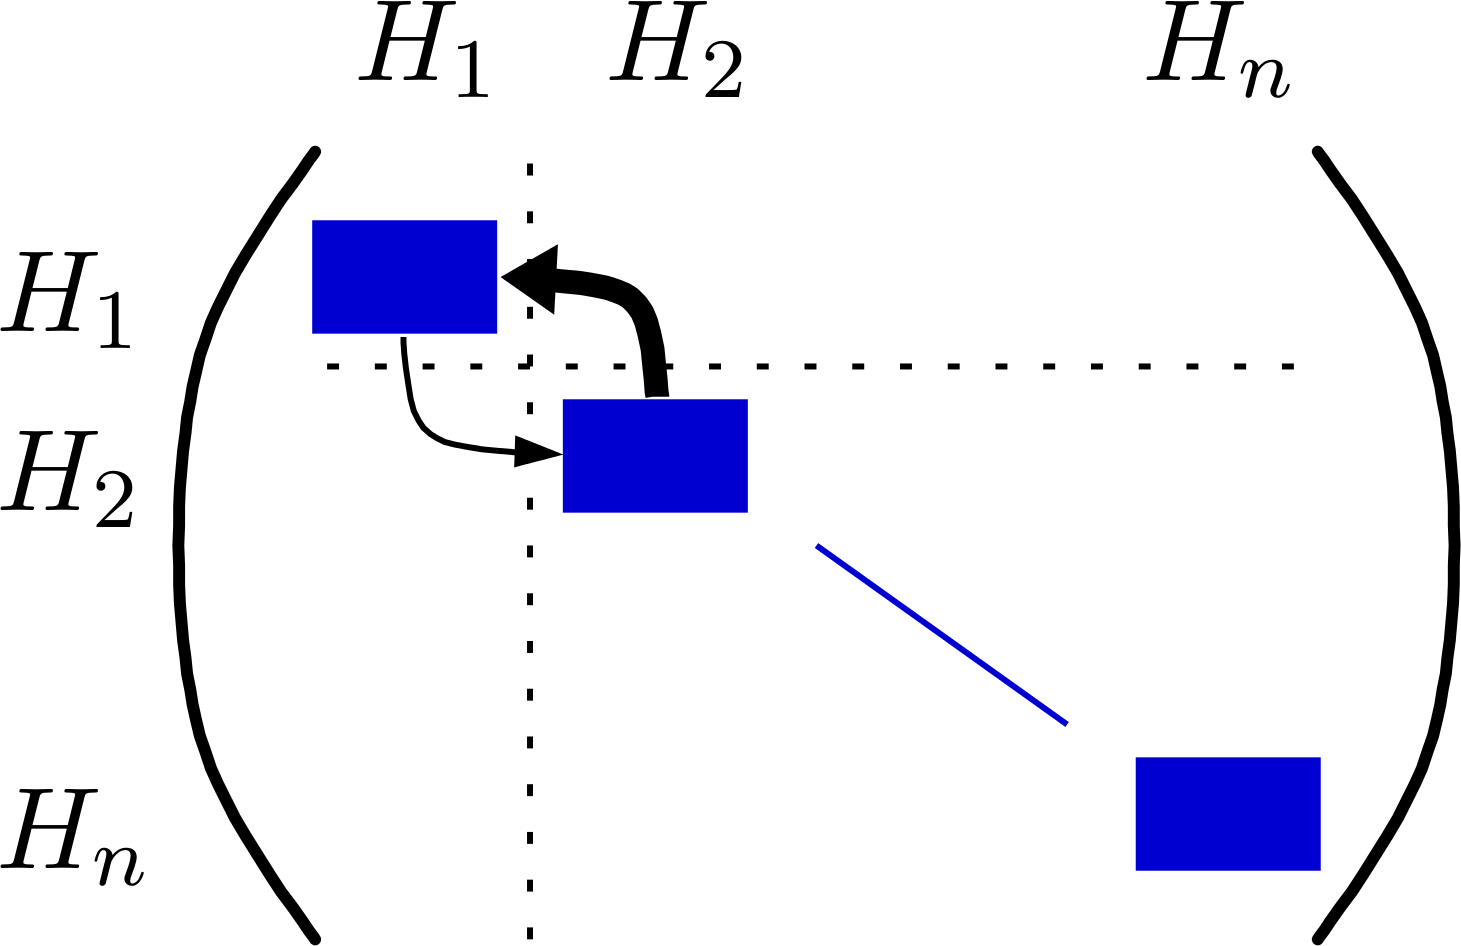
\includegraphics[width=0.45\textwidth]{matrix-structure-1} \hfill $\hphantom{1}$
%    %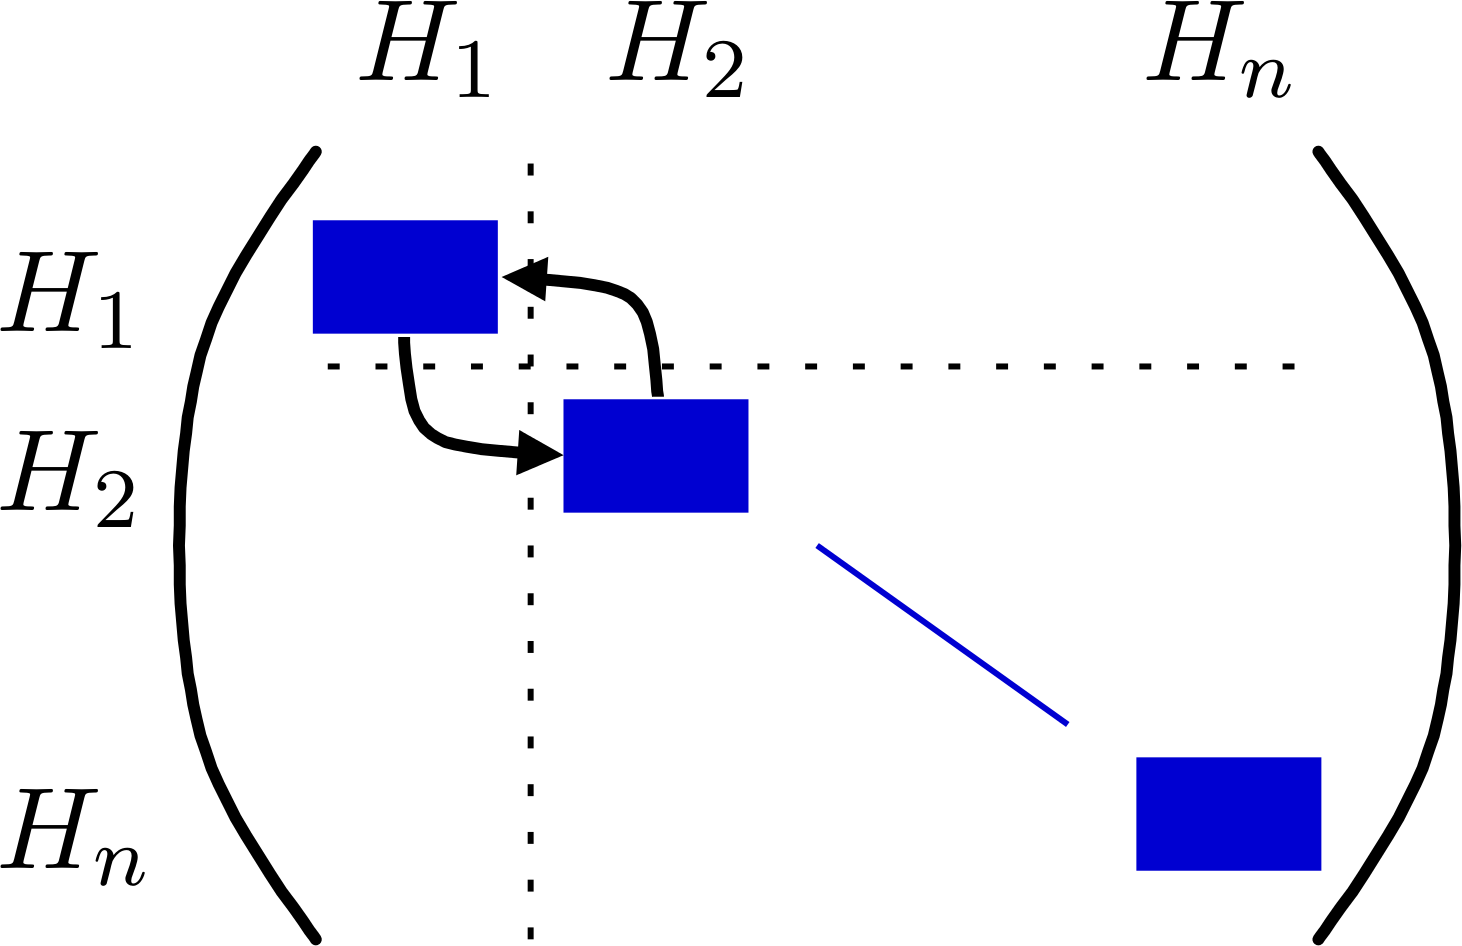
\includegraphics[width=0.45\textwidth]{matrix-structure-2}
%   \end{center}
%  \end{block}
% %  \vspace*{-0.4cm}
% 
% \end{frame}
% 
% 
% \begin{frame}{Parallelization}
%  \begin{block}{Scaling of Solution Variables}
%   \begin{itemize}
%    \item Exponential decay with energy: $f(E_i) \sim \exp(- \frac{E_i}{k_\mathrm{B} T})$
%    \item Rescale unknowns: $\tilde{f}(E_i) = \exp( \frac{E_i}{k_\mathrm{B} T}) f(E_i)$
%    \item New system: $\tilde{\matrix A} \tilde{\vector x} = \matrix A \matrix D \matrix D^{-1} \vector x = \vector b$
%    \item {\color{white} Row normalization: $\hat{\matrix A} \tilde{\vector x} = \matrix P \tilde{\matrix A} \tilde{\vector x} = \matrix P \vector b$}
%   \end{itemize}
%   \begin{center}
%    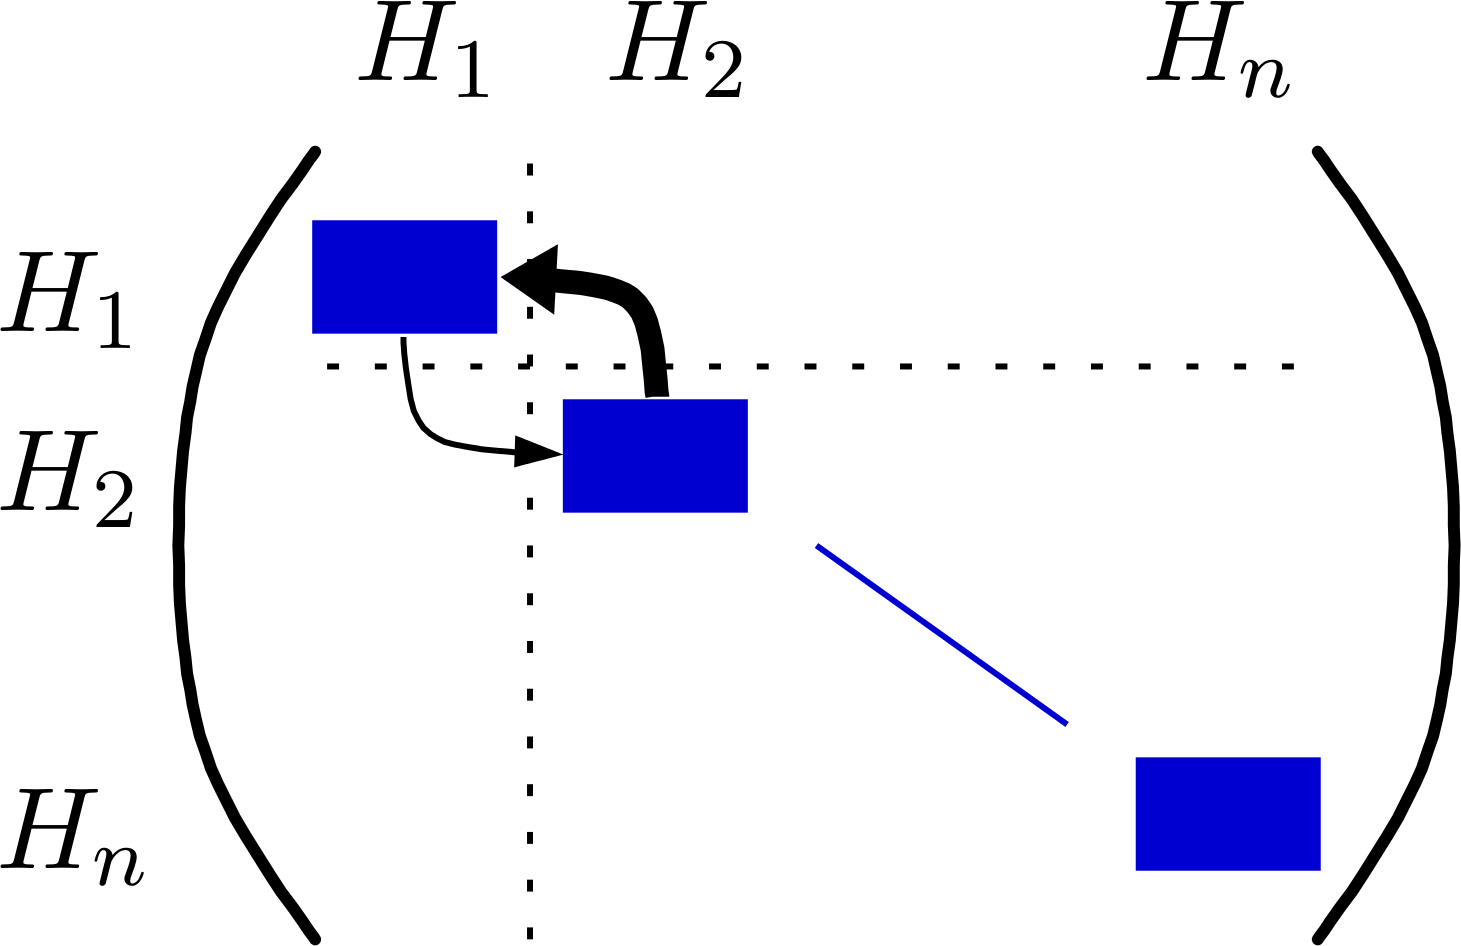
\includegraphics[width=0.45\textwidth]{matrix-structure-1} \hfill
%    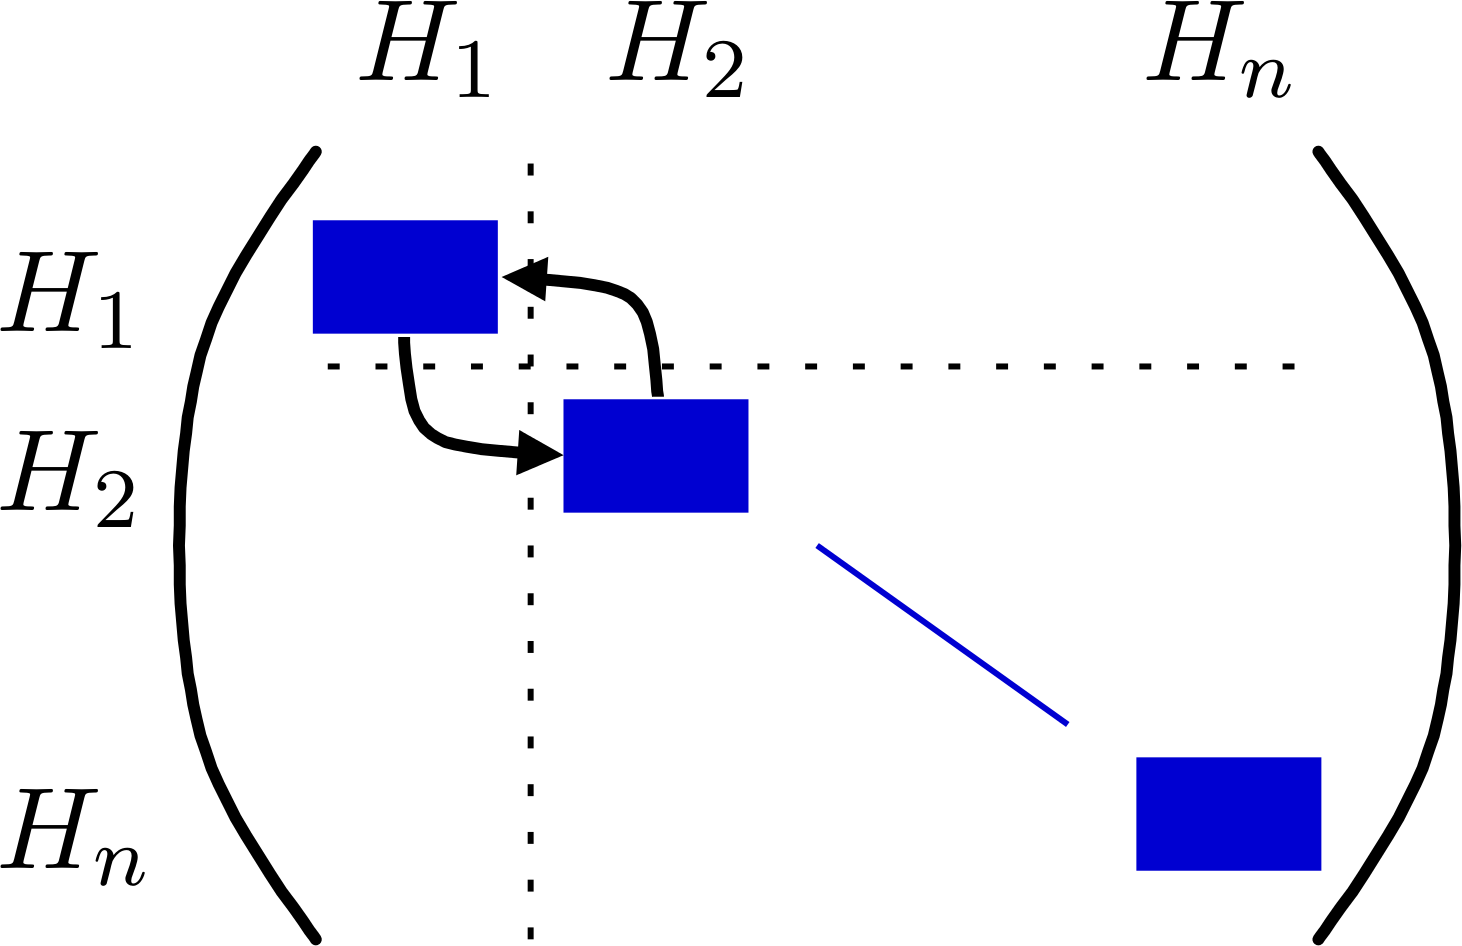
\includegraphics[width=0.45\textwidth]{matrix-structure-2}
%   \end{center}
%  \end{block}
% %  \vspace*{-0.4cm}
% 
% \end{frame}


\begin{frame}{Parallelization}
 \begin{block}{Scaling of Solution Variables}
  \begin{itemize}
   \item Exponential decay with energy: $f(E_i) \sim \exp(- \frac{E_i}{k_\mathrm{B} T})$
   \item Rescale unknowns: $\tilde{f}(E_i) = \exp( \frac{E_i}{k_\mathrm{B} T}) f(E_i)$
   \item New system: $\tilde{\matrix A} \tilde{\vector x} = \matrix A \matrix D \matrix D^{-1} \vector x = \vector b$
   \item Row normalization: $\hat{\matrix A} \tilde{\vector x} = \matrix P \tilde{\matrix A} \tilde{\vector x} = \matrix P \vector b$
  \end{itemize}
  \begin{center}
   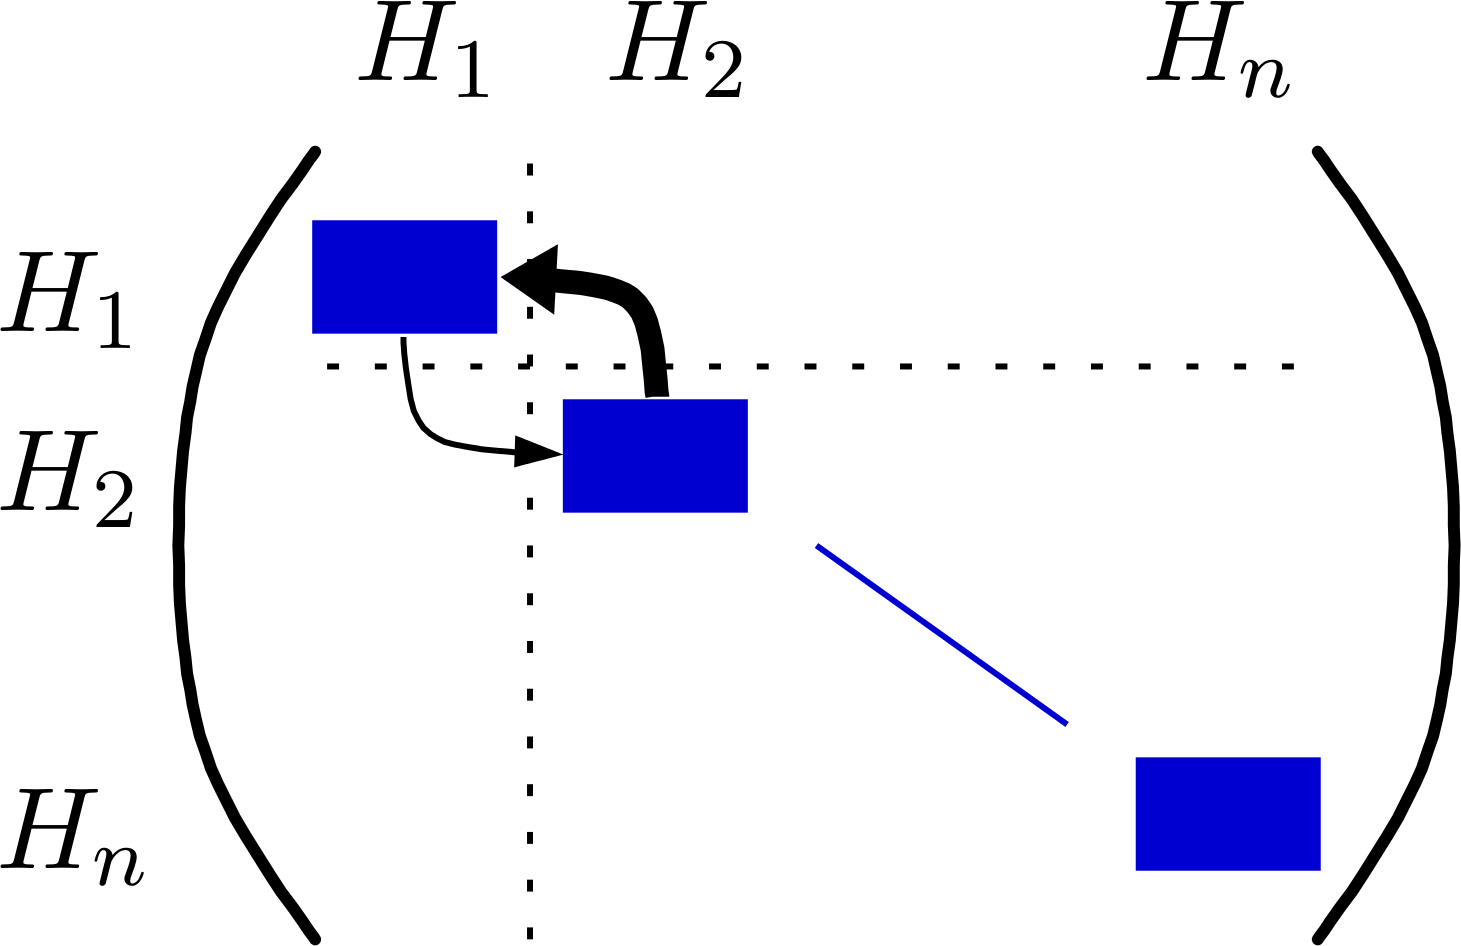
\includegraphics[width=0.45\textwidth]{matrix-structure-1} \hfill
   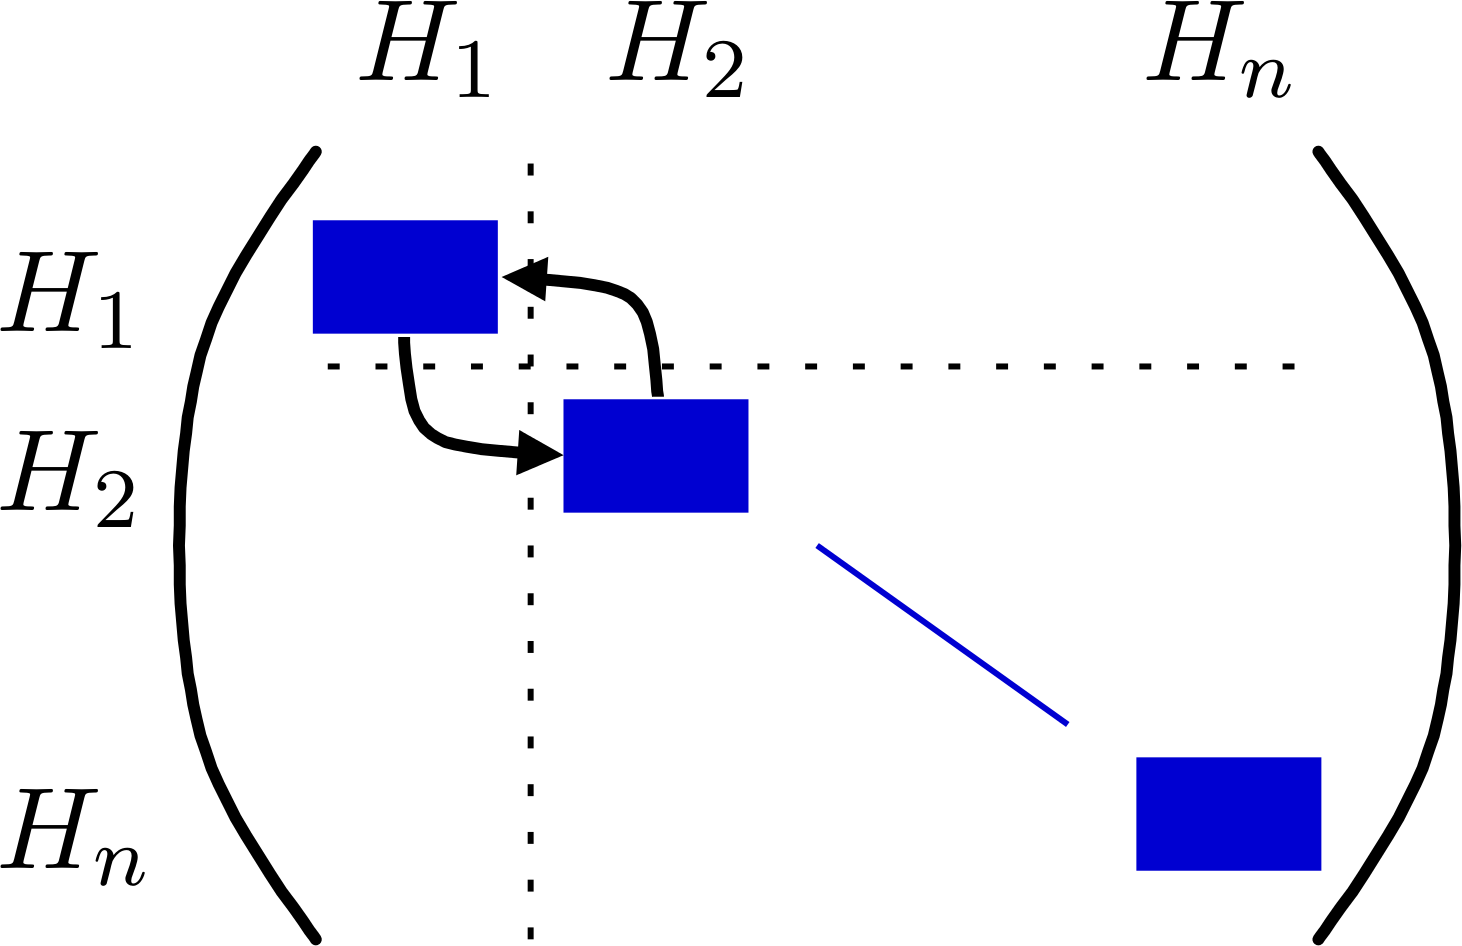
\includegraphics[width=0.45\textwidth]{matrix-structure-2}
  \end{center}
 \end{block}
%  \vspace*{-0.4cm}

\end{frame}




\begin{frame}{Parallelization}
  \vspace{-1.25cm}
  \begin{center}
   Benchmark results for a FinFET (INTEL Core i7 960, NVIDIA GTX 580) \\
   \vspace*{0.5cm}
  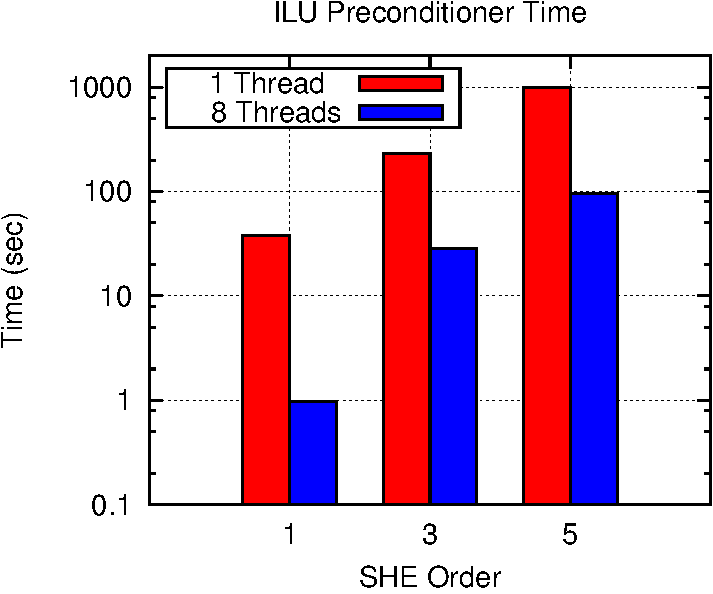
\includegraphics[width=0.48\textwidth]{mosfet-precondtimes} \hspace*{0.2cm}
  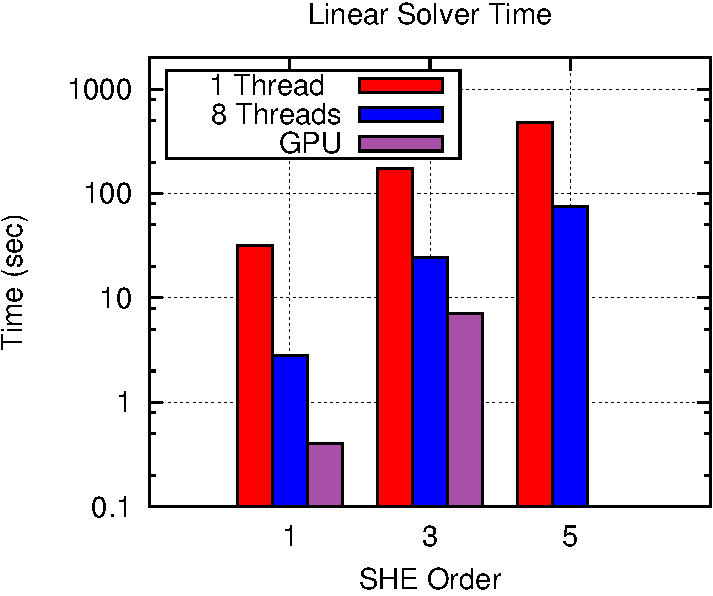
\includegraphics[width=0.48\textwidth]{mosfet-solvertimes}
  \end{center}
\end{frame}

\begin{frame}{Parallelization}
  \begin{center}
   Benchmark results for a FinFET (INTEL Core i7 960, NVIDIA GTX 580) \\
   \vspace*{0.5cm}
   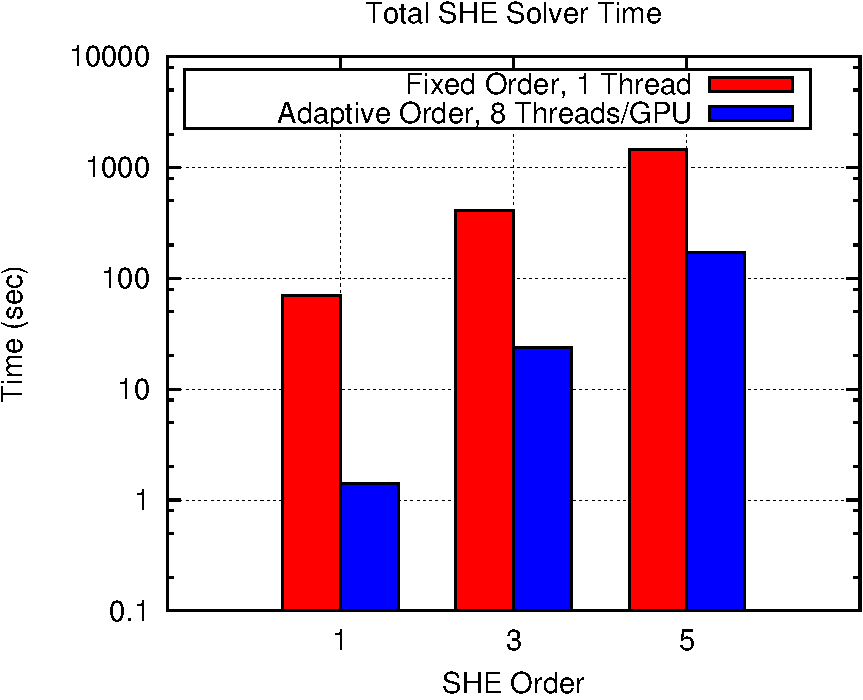
\includegraphics[width=0.7\textwidth]{mosfet-totaltimes}
  \end{center}
\end{frame}


%%%%%%%%%%% Part 2: Outlook to distributed memory %%%%%%%%%%%%%%


\begin{frame}{Part 2}
 \begin{center}
  Current Work: \\
  Development of a Parallel Preconditioner \\ 
  for (Heterogeneous) Distributed Memory Machines
 \end{center} 
 \vspace*{1cm}
 \begin{center}
  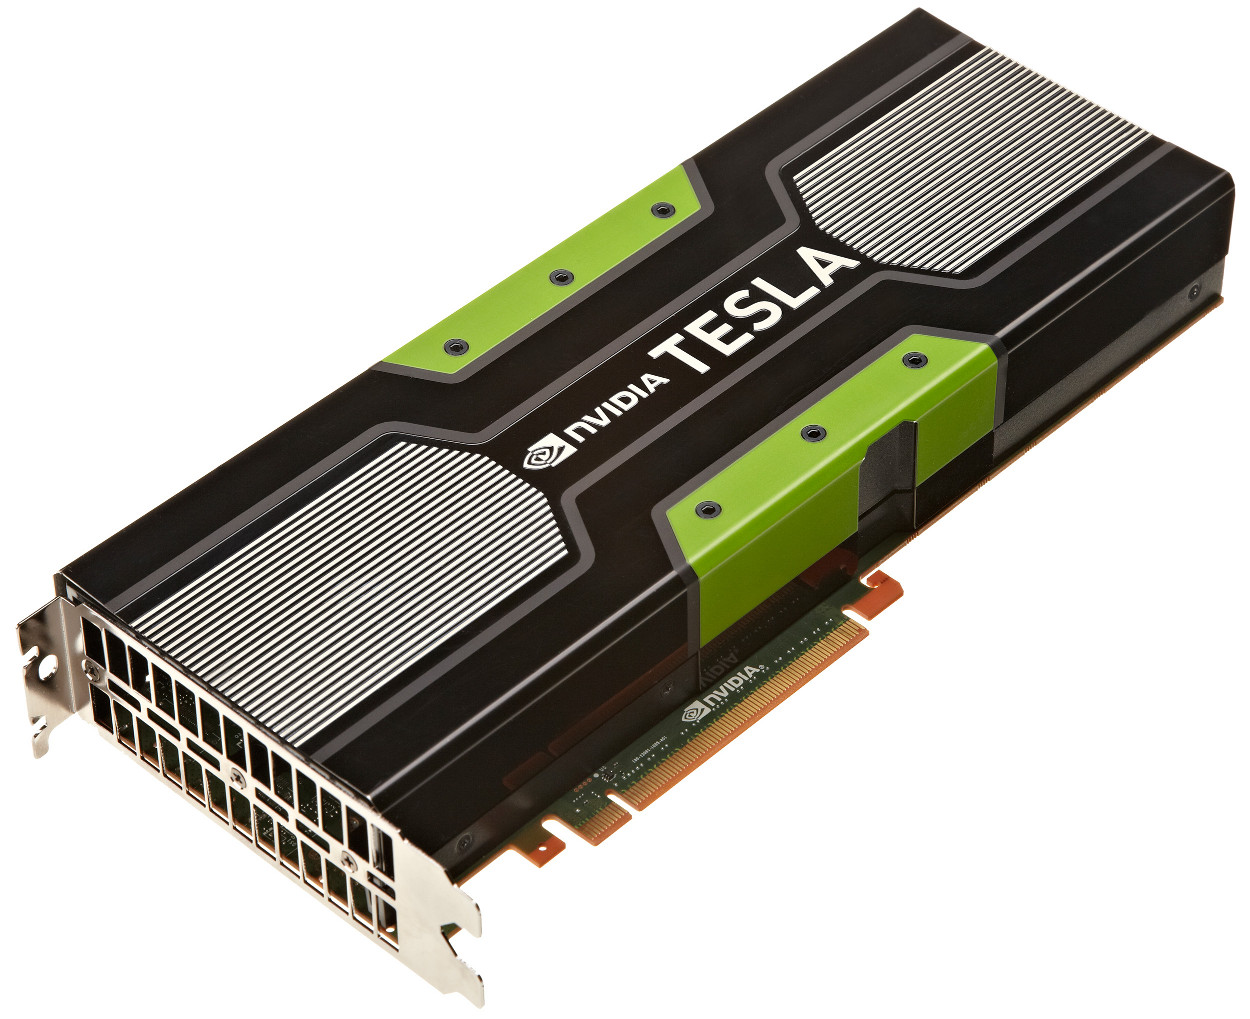
\includegraphics[width=0.25\textwidth]{figures/TeslaK20} \hfill
  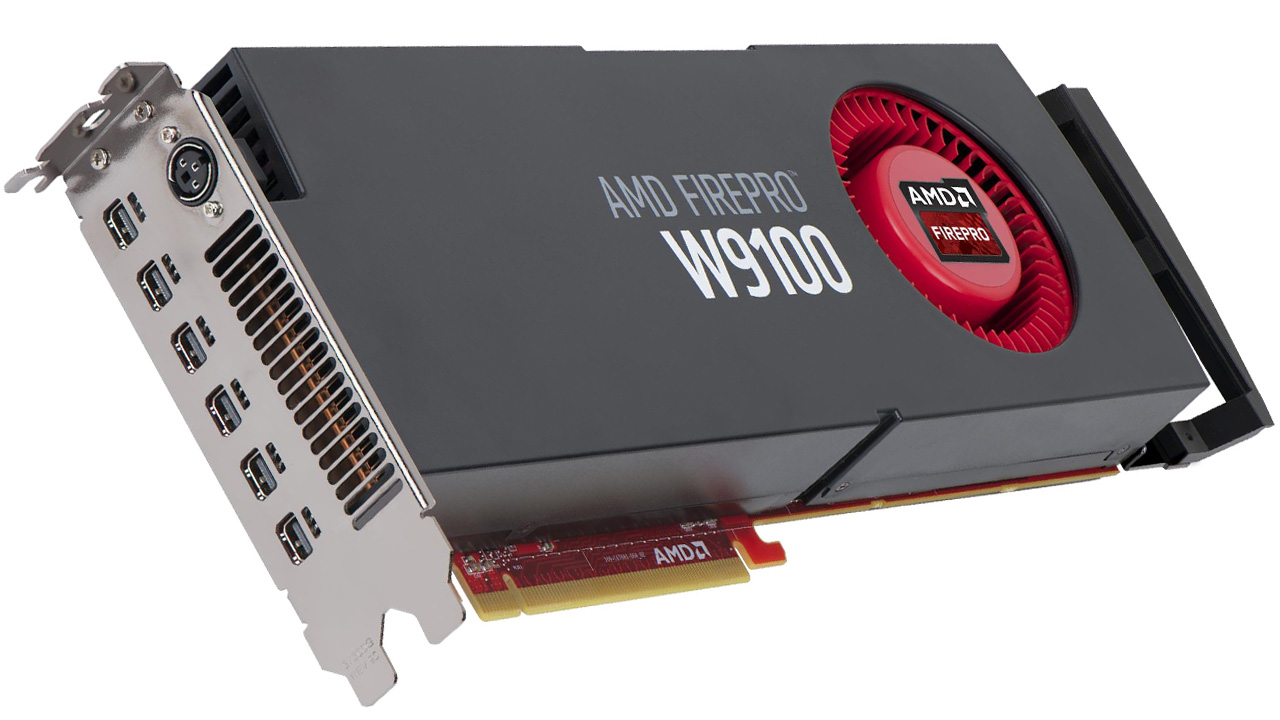
\includegraphics[width=0.3\textwidth]{figures/w9100} \hfill
  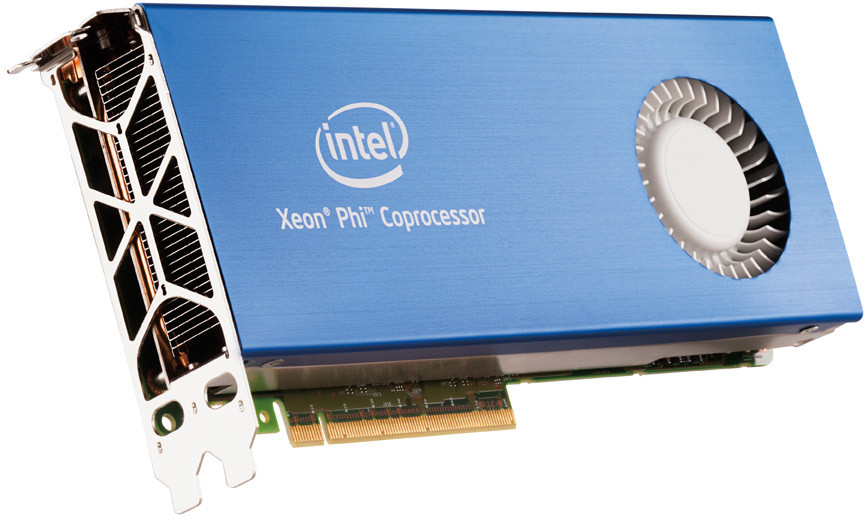
\includegraphics[width=0.3\textwidth]{figures/xeon-phi}
 \end{center}

\end{frame}


\begin{frame}{Distributed SHE}

  \begin{center}
    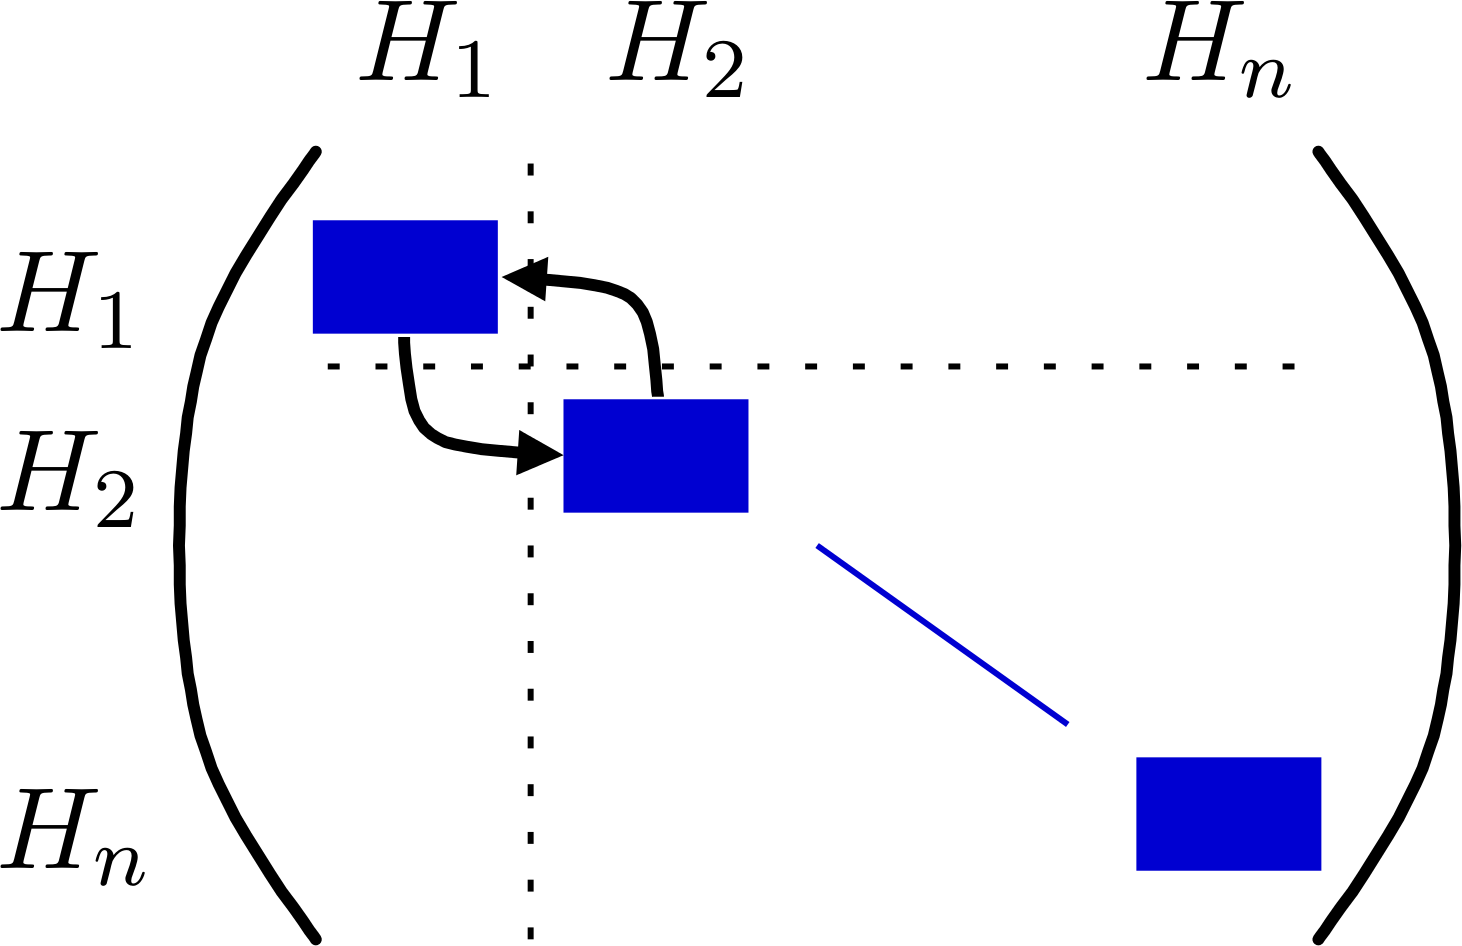
\includegraphics[width=0.45\textwidth]{matrix-structure-2}
  \end{center}

  \pause
  
  \begin{block}{Blueprint}
   \begin{itemize}
    \item Keep block-Jacobi based on total energies
    \item Map total energies to MPI ranks
    \item Requires fine-grained parallel preconditioner per block
   \end{itemize}
  \end{block}
  
\end{frame}



\begin{frame}[fragile]{Parallel ILU}

\begin{minipage}{0.45\textwidth}
  Sequential \\
  \lstinline|for i=2..n| \\
  \lstinline|  for k=1..i-1, (i,k) in A| \\
  \hspace*{0.7cm}$a_{ik} =  a_{ik}/a_{kk}$ \\
  \hspace*{0.7cm}\lstinline|for j=k+1..n, (i,j) in A| \\
  \hspace*{1cm}$a_{ij} =  a_{ij} - a_{ik}a_{kj}$ \\
\end{minipage} \hfill
\begin{minipage}{0.5\textwidth}
  Parallel \\
  \lstinline|for (sweep = 1, 2, ...)| \\
  \lstinline|  parallel for (i,j) in A| \\
  \lstinline|    if (i > j)| \\ 
  \hspace*{1cm}$l_{ij} =  (a_{ij} - \sum_{k=1}^{j=1} l_{ik}u_{kj}) / u_{jj}$ \\
  \lstinline|    else| \\
  \hspace*{1cm}$u_{ij} =  a_{ij} - \sum_{k=1}^{=1} l_{ik}u_{kj}$
\end{minipage}


  \begin{block}{Fine-Grained Parallel ILU Setup}
   \begin{itemize}
    \item Proposed by Chow and Patel (SISC, vol.~37(2)) for CPUs and MICs
    \item Massively parallel (one thread per row)
   \end{itemize}
  \end{block}
  
  \pause
  
  \begin{block}{Preconditioner Application}
   \begin{itemize}
    \item Truncated Neumann series:
     \begin{align*} \mathbf{L}^{-1} \approx \sum_{k=0}^K (\mathbf{I} - \mathbf{L})^k, \quad \mathbf{U}^{-1} \approx \sum_{k=0}^K (\mathbf{I} - \mathbf{U})^k \end{align*}
    %\item Exact triangular solves not necessary
   \end{itemize}
  \end{block}

\end{frame}

% 
% \begin{frame}{Parallel ILU}
%   \begin{center}
%     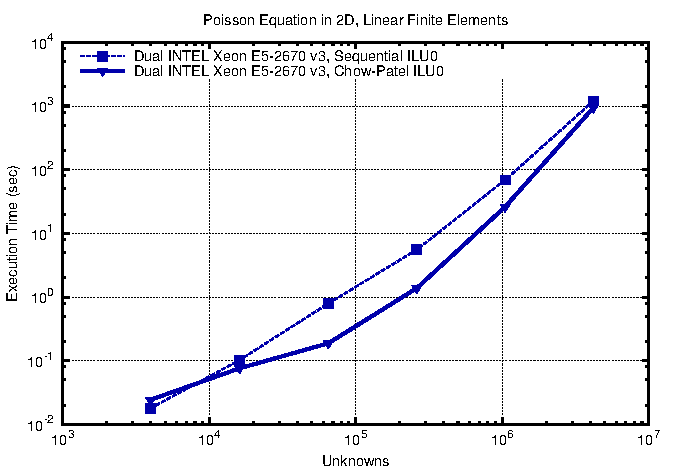
\includegraphics[width=0.95\textwidth]{ilu-2d-1}
%   \end{center}
% \end{frame}
% 
% \begin{frame}{Parallel ILU}
%   \begin{center}
%     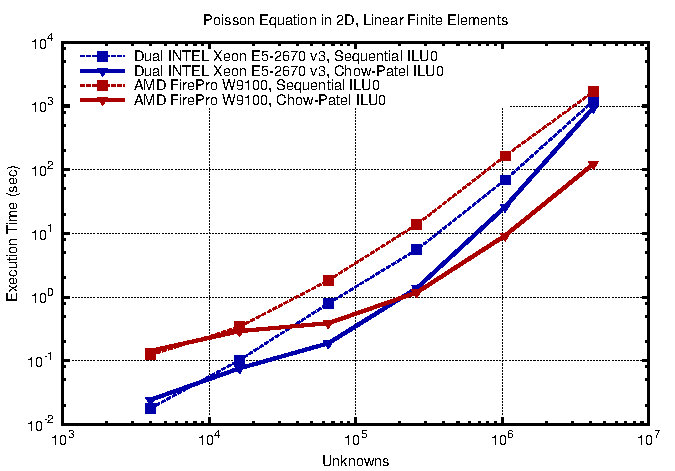
\includegraphics[width=0.95\textwidth]{ilu-2d-2}
%   \end{center}
% \end{frame}
% 
% \begin{frame}{Parallel ILU}
%   \begin{center}
%     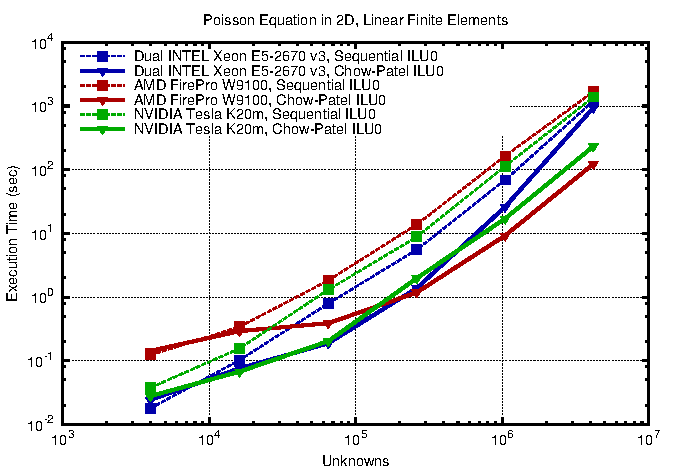
\includegraphics[width=0.95\textwidth]{ilu-2d-3}
%   \end{center}
% \end{frame}

\begin{frame}{Parallel ILU}
  \begin{center}
    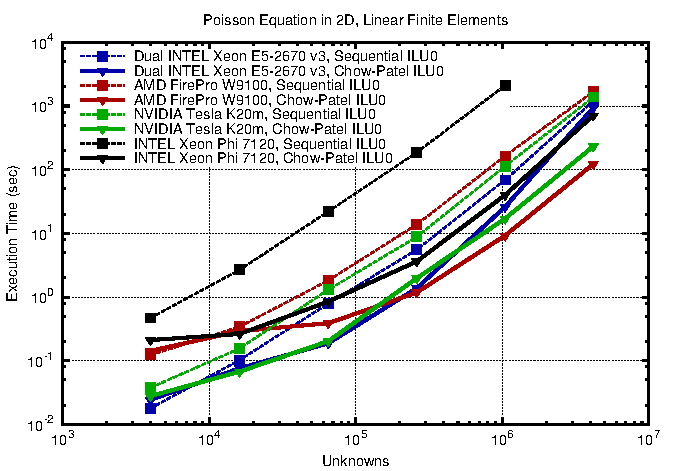
\includegraphics[width=0.95\textwidth]{ilu-2d-4}
  \end{center}
\end{frame}




%%

\begin{frame}{Conclusion}

  \begin{block}{SHE Method}
   \begin{itemize}
    \item Viable alternative to Monte Carlo
    \item Full 3D device simulations possible
    \item Convergence behavior similar to drift-diffusion model
    \item Open source simulator: ViennaSHE
   \end{itemize}
  \end{block}
  
  \pause
  
  \begin{block}{Large-Scale Solution}
   \begin{itemize}
    \item Physics-based block-Jacobi preconditioner
    \item Replication of spatial mesh on all MPI ranks
    \item Fine-grained parallel ILU
    \item Combine functionality in PETSc and ViennaCL libraries
   \end{itemize}
  \end{block}
  
\end{frame}


\end{document}

